% !TEX program = xelatex
% Options for packages loaded elsewhere
\PassOptionsToPackage{unicode}{hyperref}
\PassOptionsToPackage{hyphens}{url}
%
\documentclass[
  12pt
]{article}
\usepackage[margin=1in]{geometry}
\usepackage{amsmath,amssymb}
\usepackage{graphicx}
\usepackage{etoolbox}
\AtBeginEnvironment{tabular*}{\small}
\AtBeginEnvironment{longtable}{\small}
\usepackage{tikz}
\usetikzlibrary{arrows.meta,shapes.geometric}
\usepackage{lmodern}
\usepackage{iftex}
\ifPDFTeX
  \usepackage[T1]{fontenc}
  \usepackage[utf8]{inputenc}
  \usepackage{textcomp} % provide euro and other symbols
\else % if luatex or xetex
  \usepackage{unicode-math}
  \defaultfontfeatures{Scale=MatchLowercase}
  \defaultfontfeatures[\rmfamily]{Ligatures=TeX,Scale=1}
\fi
% Use upquote if available, for straight quotes in verbatim environments
\IfFileExists{upquote.sty}{\usepackage{upquote}}{}
\IfFileExists{microtype.sty}{% use microtype if available
  \usepackage[]{microtype}
  \UseMicrotypeSet[protrusion]{basicmath} % disable protrusion for tt fonts
}{}
\makeatletter
\@ifundefined{KOMAClassName}{% if non-KOMA class
  \IfFileExists{parskip.sty}{%
    \usepackage{parskip}
  }{% else
    \setlength{\parindent}{0pt}
    \setlength{\parskip}{6pt plus 2pt minus 1pt}}
}{% if KOMA class
  \KOMAoptions{parskip=half}}
\makeatother
\usepackage{xcolor}
\IfFileExists{xurl.sty}{\usepackage{xurl}}{} % add URL line breaks if available
\IfFileExists{bookmark.sty}{\usepackage{bookmark}}{\usepackage{hyperref}}
\hypersetup{
  hidelinks,
  pdfcreator={LaTeX via pandoc}}
\urlstyle{same} % disable monospaced font for URLs
\usepackage{longtable,booktabs,array}
\usepackage{calc}
\usepackage{needspace} % keep table captions with their tables
% Correct order of tables after \paragraph or \subparagraph
\usepackage{etoolbox}
\makeatletter
\patchcmd\longtable{\par}{\if@noskipsec\mbox{}\fi\par}{}{}
\makeatother
% Allow footnotes in longtable head/foot
\IfFileExists{footnotehyper.sty}{\usepackage{footnotehyper}}{\usepackage{footnote}}
\makesavenoteenv{longtable}
\setlength{\emergencystretch}{3em} % prevent overfull lines
\providecommand{\tightlist}{%
  \setlength{\itemsep}{0pt}\setlength{\parskip}{0pt}}
\setcounter{secnumdepth}{-\maxdimen} % remove section numbering
\ifLuaTeX
  \usepackage{selnolig}  % disable illegal ligatures
\fi

\author{}
\date{}

\begin{document}

\hypertarget{factor-validation-of-activities}{%
\subsection{Factor Validation of Activities}\label{factor-validation-of-activities}}

We examine the empirical correlates of everyday cultural practice by analyzing past-year participation frequencies across 20 distinct activities spanning institutional highbrow arts, commercial entertainment, domestic tasks, and solitary leisure routines. Because these responses are recorded on an ordinal seven-point frequency scale, we estimate principal components on the polychoric correlation matrix using varimax rotation to establish a preliminary exploratory assignment of items to factors. The three-component solution accounts for 63.2 percent of total variance, supported by a Kaiser-Meyer-Olkin sampling adequacy metric of .955 (Table 1).\footnote{Complete responses on all 20 items are available for 1,243 respondents, who form the analytic sample for all measurement models.} 

Substantively, the orthogonal solution uncovers a structural division between public, institutionalized cultural practices and private, domestic routines. Fourteen items coalesce into an expansive public arts factor, uniting traditional fine arts (symphonies, art galleries, theatrical performances) with broadly attended public events (festivals, movies, sporting events). Three items---taking walks, regular exercise or yoga, and literary reading---cluster into an independent solitary leisure dimension. Three remaining practices (gardening, home or automobile repair, and dining at fast-food restaurants) define a residual practical-domestic dimension.\footnote{We also estimated an exploratory factor analysis with direct oblimin rotation on the same polychoric matrix (Table A1). The oblique model fits the 20 items adequately ($\chi^2(133) = 290.8$, $p < .001$, $\text{TLI} = .911$, $\text{RMSEA} = .080$ $[.076, .084]$). Under direct oblimin, the public arts factor remains intact, but the secondary dimensions lose coherence. Assigning items based on highest loadings shifts literary reading, gardening, and home repair onto the arts factor, isolating fast food as a single-item residual. Forcing that assignment into confirmatory models yields inadmissible solutions characterized by negative residual variances and latent correlations exceeding unity. Because the oblique factor correlations in the exploratory solution are small (.19 between arts and leisure, .15 between arts and residual, and .01 between leisure and residual), the orthogonal and oblique orientations differ minimally in practice, and nothing in the data privileges one rotation over the other.}

We evaluate the target structure against more parsimonious alternatives using confirmatory factor analysis with diagonally weighted least squares (WLSMV estimation, N = 1,243; Table 2), which relaxes the varimax orthogonality assumption by allowing the factors to be correlated. The three-factor model outperforms more parsimonious alternatives. Forcing residual practical items onto the arts factor produces a significant decrement in fit (scaled $\Delta\chi^2(2) = 121.6$, $p < .001$), as does forcing them onto solitary leisure ($\Delta\chi^2(2) = 51.0$, $p < .001$). A single-factor model specifying a generalized omnivorousness dimension performs worst of all ($\Delta\chi^2(3) = 146.4$, $p < .001$). Although the three-factor confirmatory model fits better than any rival ($\text{CFI} = .956$, $\text{RMSEA} = .095$, $\text{SRMR} = .061$), the elevated RMSEA reflects the restrictive requirement that each practice load onto only a single factor. Everyday cultural activities naturally cross domain boundaries in ways that strict zero-loading constraints penalize.

Accordingly, we estimate an exploratory structural equation model (ESEM) using target rotation. The target matrix is built from the varimax primary-loading assignment, so each item is assigned to its primary factor and targeted toward zero on the other two. Because target rotation pulls these off-target loadings toward zero rather than fixing them, items retain small, substantively plausible cross-loadings. The ESEM achieves a good fit to the observed polychoric covariances ($\text{CFI} = .979$, $\text{RMSEA} = .074$ $[.070, .079]$, $\text{SRMR} = .035$), improving over the confirmatory baseline (scaled $\Delta\chi^2(34) = 746.7$, $p < .001$; Table 2). 

We retain the varimax targets because they align with the theoretical design of the battery, and Table A1 reports the oblimin solution of the same battery for comparison. Latent factor correlations confirm that while these three domains are distinct, they are modestly interrelated; public arts correlates positively with solitary leisure ($r = .36$) and residual domestic practices ($r = .21$), while leisure and residual practices correlate only weakly ($r = .11$; Table 3). As Table 3 shows, all fourteen public arts items maintain primary loadings between .47 and .97. Solitary leisure is anchored firmly by walking (.78) and physical exercise (.42), though exercise also displays a secondary affinity with public cultural engagement (.32). Literary reading functions as the peripheral anchor of this leisure factor across all specifications (.44 in Table 1, .21 in Table A1, and .19 in Table 3), a structural attenuation that proves central to how solitary leisure behaves across alternative operationalizations. Domestic tasks (gardening at .45, home or auto repair at .32) and fast food avoidance ($-.38$) define the residual factor, which also absorbs modest secondary loadings from institutional excursions (museums at .24, historic sites at .23) and outdoor recreation (hiking at .21). Several highbrow practices have sparse counts in the highest frequency tier, with only two respondents each for symphonies and dance performances and five for carnivals. A sensitivity analysis that collapses the top two categories of these items leaves every factor assignment unchanged and shifts the CFA fit only in the third decimal place (CFI = .955 against .956; RMSEA = .095 in both).


\Needspace{38\baselineskip}
Table 1. Varimax Loadings for the Activity Battery

\begin{longtable}[]{@{}
  >{\raggedright\arraybackslash}p{(\columnwidth - 8\tabcolsep) * \real{0.4200}}
  >{\raggedright\arraybackslash}p{(\columnwidth - 8\tabcolsep) * \real{0.1600}}
  >{\raggedright\arraybackslash}p{(\columnwidth - 8\tabcolsep) * \real{0.1400}}
  >{\raggedright\arraybackslash}p{(\columnwidth - 8\tabcolsep) * \real{0.1400}}
  >{\raggedright\arraybackslash}p{(\columnwidth - 8\tabcolsep) * \real{0.1400}}@{}}
\toprule
Item & Assigned target & Arts & Leisure & Residual \\
Museum & Arts & \textbf{0.80} & 0.21 & 0.21 \\
Art gallery & Arts & \textbf{0.83} & 0.19 & 0.20 \\
Symphony, orchestra, or opera & Arts & \textbf{0.89} & 0.06 & 0.23 \\
Carnival, fair, or amusement park & Arts & \textbf{0.83} & 0.13 & 0.01 \\
Music concert or festival & Arts & \textbf{0.84} & 0.17 & 0.02 \\
Play or musical & Arts & \textbf{0.84} & 0.09 & 0.13 \\
Library & Arts & \textbf{0.49} & 0.39 & 0.15 \\
Fancy restaurant & Arts & \textbf{0.72} & 0.26 & −0.15 \\
Dance performance & Arts & \textbf{0.89} & 0.00 & 0.15 \\
Movie theater & Arts & \textbf{0.74} & 0.23 & −0.24 \\
Attend sports & Arts & \textbf{0.79} & 0.21 & −0.07 \\
Hiking, camping, or boating & Arts & \textbf{0.52} & 0.37 & 0.32 \\
Historic site & Arts & \textbf{0.70} & 0.23 & 0.26 \\
Go to festival & Arts & \textbf{0.78} & 0.27 & 0.15 \\
Go for a walk & Leisure & −0.14 & \textbf{0.87} & 0.07 \\
Exercise or yoga & Leisure & 0.35 & \textbf{0.60} & −0.19 \\
Read a novel, poem, or play & Leisure & 0.27 & \textbf{0.44} & 0.18 \\
Gardening & Residual & 0.27 & 0.31 & \textbf{0.62} \\
Fast food & Residual & 0.21 & 0.22 & \textbf{−0.66} \\
Home auto repair & Residual & 0.38 & 0.24 & \textbf{0.49} \\
\midrule
\endhead
\bottomrule
\end{longtable}

Note. Varimax-rotated component loadings from a principal components analysis (N = 1,243). Bold entries mark each item's assigned factor. The assigned target column reports the factor on which each item is assigned in the ESEM targets. The three components together explain 63.2 percent of the variance.

\Needspace{26\baselineskip}
Table 2. Confirmatory and Exploratory Structural Models of the Activity Battery

\begin{longtable}[]{@{}
  >{\raggedright\arraybackslash}p{(\columnwidth - 12\tabcolsep) * \real{0.3000}}
  >{\raggedright\arraybackslash}p{(\columnwidth - 12\tabcolsep) * \real{0.0600}}
  >{\raggedright\arraybackslash}p{(\columnwidth - 12\tabcolsep) * \real{0.1200}}
  >{\raggedright\arraybackslash}p{(\columnwidth - 12\tabcolsep) * \real{0.0800}}
  >{\raggedright\arraybackslash}p{(\columnwidth - 12\tabcolsep) * \real{0.1000}}
  >{\raggedright\arraybackslash}p{(\columnwidth - 12\tabcolsep) * \real{0.1000}}
  >{\raggedright\arraybackslash}p{(\columnwidth - 12\tabcolsep) * \real{0.2400}}@{}}
\toprule
Model & df & Scaled $\chi^2$ & CFI & RMSEA & SRMR & Scaled $\Delta\chi^2$ (df) vs.~three-factor CFA \\
One-factor CFA & 170 & 2225.6 & .952 & .099 & .064 & 146.4 (3), p \textless{} .001 \\
Two-factor CFA, residual merged into arts & 169 & 2199.3 & .952 & .098 & .063 & 121.6 (2), p \textless{} .001 \\
Two-factor CFA, residual merged into leisure & 169 & 2120.8 & .954 & .096 & .062 & 51.0 (2), p \textless{} .001 \\
Three-factor CFA & 167 & 2051.2 & .956 & .095 & .061 & --- \\
ESEM, target rotation & 133 & 1045.1 & .979 & .074 & .035 & 746.7 (34), p \textless{} .001 \\
\midrule
\endhead
\bottomrule
\end{longtable}

Note. N = 1,243. WLSMV estimation. The three-factor CFA is nested within the ESEM's implied covariance class as the case with zero cross-loadings, so the ESEM row reports a scaled difference test against it. The ESEM degrees of freedom reflect its rotation constraints. Latent factor correlations in the three-factor CFA are .76 (arts and leisure), .68 (arts and residual), and .59 (leisure and residual). RMSEA 90\% confidence intervals are {[}.095, .102{]} (one-factor), {[}.095, .102{]} (residual into arts), {[}.093, .100{]} (residual into leisure), {[}.092, .099{]} (three-factor), and {[}.070, .079{]} (ESEM). Scaled difference tests use the Satorra-Bentler scaled statistic with per-model scaling factors.

\Needspace{38\baselineskip}
Table 3. ESEM Loadings with Target Rotation

\begin{longtable}[]{@{}
  >{\raggedright\arraybackslash}p{(\columnwidth - 8\tabcolsep) * \real{0.4200}}
  >{\raggedright\arraybackslash}p{(\columnwidth - 8\tabcolsep) * \real{0.1600}}
  >{\raggedright\arraybackslash}p{(\columnwidth - 8\tabcolsep) * \real{0.1400}}
  >{\raggedright\arraybackslash}p{(\columnwidth - 8\tabcolsep) * \real{0.1400}}
  >{\raggedright\arraybackslash}p{(\columnwidth - 8\tabcolsep) * \real{0.1400}}@{}}
\toprule
Item & Target factor & Arts & Leisure & Residual \\
Museum & Arts & \textbf{0.78} & 0.03 & 0.24 \\
Art gallery & Arts & \textbf{0.83} & −0.02 & 0.20 \\
Symphony, orchestra, or opera & Arts & \textbf{0.95} & −0.22 & 0.11 \\
Carnival, fair, or amusement park & Arts & \textbf{0.82} & 0.04 & −0.11 \\
Music concert or festival & Arts & \textbf{0.86} & 0.02 & −0.11 \\
Play or musical & Arts & \textbf{0.90} & −0.16 & 0.02 \\
Library & Arts & \textbf{0.47} & 0.16 & 0.14 \\
Fancy restaurant & Arts & \textbf{0.71} & 0.15 & −0.20 \\
Dance performance & Arts & \textbf{0.97} & −0.25 & 0.01 \\
Movie theater & Arts & \textbf{0.75} & 0.11 & −0.30 \\
Attend sports & Arts & \textbf{0.80} & 0.08 & −0.21 \\
Hiking, camping, or boating & Arts & \textbf{0.48} & 0.23 & 0.21 \\
Historic site & Arts & \textbf{0.65} & 0.11 & 0.23 \\
Go to festival & Arts & \textbf{0.78} & 0.10 & 0.04 \\
Go for a walk & Leisure & −0.22 & \textbf{0.78} & 0.12 \\
Exercise or yoga & Leisure & 0.32 & \textbf{0.42} & −0.17 \\
Read a novel, poem, or play & Leisure & 0.27 & \textbf{0.19} & 0.16 \\
Gardening & Residual & 0.23 & 0.17 & \textbf{0.45} \\
Fast food & Residual & 0.20 & 0.14 & \textbf{−0.38} \\
Home auto repair & Residual & 0.34 & 0.14 & \textbf{0.32} \\
\midrule
\endhead
\bottomrule
\end{longtable}

Note. Standardized loadings from an ESEM with target rotation (WLSMV, N = 1,243). Bold entries mark each item's assigned factor. Factor correlations: arts and leisure .36, arts and residual .21, leisure and residual .11.


\subsection{Factor Validation of Network Composition}\label{factor-validation-of-network-composition}

The position generator batteries assess personal networks across sixteen social categories, measured separately for casual acquaintances (weak ties) and close confidants (strong ties).\footnote{Gender items (knowing men, knowing women) are excluded because they display marked structural ambiguity across both relational domains. In exploratory analyses, knowing women splits nearly equally between the liberal and conservative factors in weak networks (.59 and .60), while knowing men loads heavily on both factors in weak ties (.68 and .57) and on conservative composition in strong ties (.62, alongside a .58 loading on liberal composition). In confirmatory models, retaining them lowers fit to $\text{CFI} = .896$ and $\text{RMSEA} = .116$ for weak ties and $\text{CFI} = .918$ and $\text{RMSEA} = .105$ for strong ties. Re-estimating regression models without the four gender items leaves every substantive finding and significance verdict intact, with no network coefficient shifting by more than .049.} Rather than collapsing social ties into an omnibus index of network diversity, the measurement model uncovers three distinct relational structures across both relational spheres: a generalized breadth of ties spanning ethnic, geographic, and socioeconomic boundaries (Network Variety), and two distinct channels of partisan homophily (Liberal Composition and Conservative Composition). This separation confirms that demographic bridging and ideological sorting operate as distinct relational dynamics; maintaining connections across varied social strata does not imply alignment with a particular political camp.

Social diversity and political sorting rarely occupy hermetically sealed environments. Conventional confirmatory factor models, which impose strict zero-loading restrictions by forcing each social position onto a single factor, fit the data poorly and mischaracterize everyday network topology (Table A2).\footnote{In simple-structure confirmatory models, freeing residual covariances between polar opposites (very liberal with very conservative, little church with lots of church, and city with rural) modestly improves fit (Table A2). Under the target-rotated ESEM, however, secondary cross-loadings absorb this bipolarity, rendering those residual covariances redundant and producing numerical instability in strong-tie estimation. We therefore retain the target ESEM without residual covariances.} By penalizing the natural secondary affinities that exist among demographic and political identities, strict confirmatory models artificially force shared social spaces into the latent factor correlations, inflating the overlap between network variety and liberal composition to over .80 and inducing severe collinearity. Estimating exploratory structural equation models (ESEM) with target rotation resolves this distortion (Table 4). By permitting positions to display modest, substantively meaningful secondary affinities, the ESEM achieves a good fit ($\text{CFI} \ge .975$, $\text{RMSEA} \le .069$, $\text{SRMR} \le .033$), showing that while demographic diversity and progressive sorting intersect in everyday networks, they remain distinct, moderately related dimensions ($r \approx .50$).

The pattern of secondary loadings in Table 4 reveals a meaningful shift in how racial diversity and political sorting operate across levels of intimacy. In casual acquaintance networks, minoritized racial and ethnic ties (Black and Hispanic or Latine acquaintances) straddle both network variety and progressive political composition. This pattern reflects the institutional organization of everyday social life; for many Americans, casual contact across racial lines occurs within progressive urban, educational, or professional environments. In close personal networks, by contrast, these same ties anchor structural variety almost exclusively. When Americans form close, confiding bonds across racial lines, those ties represent genuine cross-boundary social bridging rather than incidental proximity to progressive politics. Conservative composition, meanwhile, exhibits a starkly consolidated relational boundary across both weak and strong spheres; it is anchored exclusively by church attendance, political conservatism, rural residence, and White ties. White ties also display secondary affinities with liberal networks, capturing the partisan divide within the majority population, whereas conservative homophily remains structurally insular and segregated from ethnic diversity.

All three network dimensions achieve high internal reliability across both tie types, with model-implied omegas ranging from .88 to .94 (Table 4). In the structural models that follow, both the network and activity blocks are the target-rotated ESEMs, with their loadings fixed at the target values, and the confirmatory factors serve as a comparison (Table A2).\footnote{We do not estimate a joint model that links the weak and strong factors in the main analysis. Without residual covariances between matching items, the joint model does not converge, and with them it converges only at a weakly identified solution in which the weak and strong variety factors have a disturbance correlation of .84 and their leisure paths cancel. The separate models are therefore the basis for inference in both tie types.}

\Needspace{30\baselineskip}
Table 4. Standardized Loadings from the Target-Rotated ESEM of the Weak-Tie and Strong-Tie Batteries

\begin{tabular*}{\textwidth}{@{\extracolsep{\fill}}>{\raggedright\arraybackslash}p{0.34\textwidth} >{\raggedleft\arraybackslash}p{0.09\textwidth} >{\raggedleft\arraybackslash}p{0.09\textwidth} >{\raggedleft\arraybackslash}p{0.09\textwidth} >{\raggedleft\arraybackslash}p{0.09\textwidth} >{\raggedleft\arraybackslash}p{0.09\textwidth} >{\raggedleft\arraybackslash}p{0.09\textwidth}@{}}
\toprule
 & \multicolumn{3}{c}{Weak ties} & \multicolumn{3}{c}{Strong ties} \\
\cmidrule(lr){2-4}\cmidrule(lr){5-7}
Item & Variety & Liberal & Conservative & Variety & Liberal & Conservative \\
\midrule
Asian people & \textbf{0.61} & 0.33 & $-$0.03 & \textbf{0.73} & 0.15 & $-$0.06 \\
Second home & \textbf{0.50} & $-$0.03 & 0.34 & \textbf{0.56} & $-$0.09 & 0.31 \\
Born elsewhere & \textbf{0.48} & 0.38 & 0.02 & \textbf{0.70} & 0.19 & $-$0.04 \\
MENA people & \textbf{0.77} & 0.15 & 0.00 & \textbf{0.88} & 0.02 & $-$0.02 \\
NHPI people & \textbf{0.93} & $-$0.04 & $-$0.06 & \textbf{0.93} & $-$0.08 & $-$0.05 \\
American Indian people & \textbf{0.84} & $-$0.12 & 0.06 & \textbf{0.85} & $-$0.14 & 0.09 \\
LGBTQ people & 0.03 & \textbf{0.80} & $-$0.07 & 0.24 & \textbf{0.65} & $-$0.10 \\
Little church & $-$0.11 & \textbf{0.58} & 0.32 & $-$0.07 & \textbf{0.54} & 0.36 \\
Very liberal & $-$0.02 & \textbf{0.78} & 0.05 & 0.08 & \textbf{0.81} & $-$0.01 \\
Hispanic or Latine people & 0.32 & \textbf{0.54} & 0.01 & \textbf{0.59} & 0.27 & $-$0.04 \\
Black people & 0.36 & \textbf{0.36} & 0.16 & \textbf{0.55} & 0.18 & 0.15 \\
City people & 0.30 & \textbf{0.44} & 0.07 & 0.35 & \textbf{0.36} & 0.12 \\
Lots of church & 0.22 & $-$0.02 & \textbf{0.67} & 0.29 & $-$0.09 & \textbf{0.63} \\
Very conservative & 0.11 & $-$0.20 & \textbf{0.90} & 0.14 & $-$0.20 & \textbf{0.81} \\
White people & $-$0.19 & 0.41 & \textbf{0.68} & $-$0.15 & 0.36 & \textbf{0.72} \\
Rural people & $-$0.07 & 0.11 & \textbf{0.61} & $-$0.05 & 0.16 & \textbf{0.60} \\
\bottomrule
\end{tabular*}

Note. Standardized loadings from exploratory structural equation models with target rotation (WLSMV, polychoric; N = 1,258 per battery). Bold entries are the primary loadings from the target, and all other loadings are estimated rather than fixed at zero. Gender items are excluded. Factor correlations are .52 (variety and liberal), .46 (variety and conservative), and .47 (liberal and conservative) for weak ties, and .48, .54, and .34 in the same order for strong ties. Item labels are abbreviated from the variable names; MENA is Middle Eastern or North African, and NHPI is Native Hawaiian or Pacific Islander.


\subsection{Structural Models of Activity Participation}\label{structural-models-of-activity-participation}

To evaluate how network variety and ideological composition relate to cultural participation, we estimate structural equation models separately for weak and strong ties. Each model pairs the three network factors (variety, liberal composition, and conservative composition) with the three activity factors (public arts, solitary leisure, and practical-domestic residual activity), and both measurement blocks are target-rotated exploratory structural equation models in which secondary loadings are retained.\footnote{The loadings are fixed at the values from an external target rotation, so their sampling error does not enter the structural standard errors. The factor correlations implied by these loadings depend on the rotation chosen, and a split-half comparison with an oblimin rotation is reported in Table A3. Because these survey data are cross-sectional, the paths describe patterns of relational association rather than causal order. The residual factor has modest reliability ($\omega = .55$), so its paths should be read cautiously.} Gender, race and ethnicity, childhood arts exposure, household income, age in years, and political ideology (1 to 7) predict every network and activity factor. Education enters as a single ordinal variable running from high school or less (1) to graduate credentials (4). Estimated on complete cases (N = 1,227) using weighted least squares with mean and variance adjustment (WLSMV), both models converge and yield positive definite covariance matrices. Fit is adequate but weaker than that of the confirmatory and ESEM measurement models ($\text{CFI} = .891$, $\text{RMSEA} = .058$, $\text{SRMR} = .075$ for weak ties; $\text{CFI} = .862$, $\text{RMSEA} = .066$, $\text{SRMR} = .086$ for strong ties).

Network variety is the main relational channel for public arts attendance in both tie types, with standardized paths of .19 for weak ties and .25 for strong ties (both $p < .001$; Table 5). Liberal and conservative composition each carry small positive paths on arts, between .04 and .08, all significant at $p < .001$. The negative liberal coefficient that organized our earlier account of arts participation does not appear under these fixed-loading models. The ordinary least squares models on the polychoric factor scores do reproduce it, with weak-tie liberal composition at $-.12$ in the full model (Table A4, $p < .001$). The sign of that path therefore depends on the measurement model, and we do not treat the suppression account as settled.\footnote{Under an oblimin rotation of the same specification, estimated separately in random halves of the sample (seed 4217), the variety paths on arts stay positive in every half for both tie types, while the weak liberal path on arts is near zero and changes sign across halves. We therefore treat the liberal path on arts as unstable. The liberal paths on solitary leisure are positive under both rotations.}

Solitary leisure runs through liberal composition rather than variety. Weak liberal composition (.20) and strong liberal composition (.22) are positive and significant at $p < .001$, while network variety and conservative composition are null in both tie types (weak variety .06, $p = .19$; strong variety $-.05$, $p = .27$). Practical-domestic residual activity shows smaller and less consistent paths, with variety positive in both tie types (.10 for weak ties, $p = .009$; .11 for strong ties, $p = .006$) and weak liberal composition negative and marginal ($-.09$, $p = .06$).

The labeled models also decompose the sociodemographic and background effects into direct and network-mediated components (Tables 10 and 11). Education has a total standardized effect of .35 on arts participation in both tie models, of which about .05 runs through weak ties and about .07 through strong ties. Childhood arts exposure has a total effect of .27, of which about .05 (weak) and .07 (strong) runs through network composition, and the remainder is direct. Political conservatism has a total effect of .09 on arts. Its direct path is about .07 for weak ties and about .05 for strong ties, and its network-mediated path is about .02 for weak ties and about .04 for strong ties, with both mediated paths significant at $p < .01$. The total effects are nearly identical across tie models, because the covariate-to-activity relations are unconstrained in both, so the tie comparison concerns how much of each total runs through the network.\footnote{The total effects differ by no more than .004 between the weak-tie and strong-tie models for every predictor and activity factor. Only the split between direct and network-mediated routes differs by tie type.}

Political conservatism's total association with solitary leisure is $-.12$ in both models ($p = .001$). Its network-mediated part runs through liberal composition and is $-.07$ for weak ties ($p = .09$) and $-.11$ for strong ties ($p = .02$), so the strong-tie channel is the one that clears conventional thresholds. Network-mediated effects are summed over the three network factors and assume that the covariates are not confounding the network-to-activity paths.

Sociodemographic patterns sit alongside these relational dynamics (Tables 6 to 9). Education predicts network variety in both tie types (.26 for weak and strong ties), and political conservatism predicts liberal composition negatively ($-.50$ weak, $-.54$ strong) and conservative composition positively (.39 weak, .43 strong). Race and ethnicity predict conservative composition most strongly: AAPI respondents show the largest negative conservative paths ($-.20$ weak, $-.25$ strong), and Black, Hispanic or Latine, and multiracial respondents show comparable negative paths. Education and childhood arts exposure predict public arts attendance in both models (education .30 and .28; childhood arts .22 and .20), while AAPI respondents report lower arts participation in both tie models ($-.07$ weak, $-.06$ strong).


Table 5. Standardized Network-to-Activity Paths from the Separate Weak-Tie and Strong-Tie Structural Models

\begin{tabular*}{\textwidth}{@{\extracolsep{\fill}}>{\raggedright\arraybackslash}p{0.36\textwidth} >{\raggedleft\arraybackslash}p{0.20\textwidth} >{\raggedleft\arraybackslash}p{0.20\textwidth} >{\raggedleft\arraybackslash}p{0.20\textwidth}@{}}
\toprule
Network factor & Arts & Solitary leisure & Residual \\
\midrule
Weak variety & \hphantom{$-$}0.19***\hphantom{} & \hphantom{$-$}0.06\hphantom{***} & \hphantom{$-$}0.10**\hphantom{*} \\
Weak liberal & \hphantom{$-$}0.05***\hphantom{} & \hphantom{$-$}0.20***\hphantom{} & $-$0.09\hphantom{***} \\
Weak conservative & \hphantom{$-$}0.04***\hphantom{} & \hphantom{$-$}0.05\hphantom{***} & $-$0.01\hphantom{***} \\
Strong variety & \hphantom{$-$}0.25***\hphantom{} & $-$0.05\hphantom{***} & \hphantom{$-$}0.11**\hphantom{*} \\
Strong liberal & \hphantom{$-$}0.04***\hphantom{} & \hphantom{$-$}0.22***\hphantom{} & $-$0.04\hphantom{***} \\
Strong conservative & \hphantom{$-$}0.08***\hphantom{} & \hphantom{$-$}0.03\hphantom{***} & \hphantom{$-$}0.01\hphantom{***} \\
\bottomrule
\end{tabular*}

Note. Standardized coefficients from separate WLSMV structural models for weak ties and strong ties (N = 1,227 each), with loadings fixed at the target rotation of each battery. Each model includes gender, education, childhood arts exposure, income, age, race and ethnicity, and political ideology as predictors of all factors. * p < .05, ** p < .01, *** p < .001.

Table 6. Sociodemographic Predictors of Weak-Tie Network Factors

\begin{tabular*}{\textwidth}{@{\extracolsep{\fill}}>{\raggedright\arraybackslash}p{0.36\textwidth} >{\raggedleft\arraybackslash}p{0.20\textwidth} >{\raggedleft\arraybackslash}p{0.20\textwidth} >{\raggedleft\arraybackslash}p{0.20\textwidth}@{}}
\toprule
Predictor & Variety & Liberal & Conservative \\
\midrule
Age (years) & $-$0.13***\hphantom{} & \hphantom{$-$}0.02\hphantom{***} & \hphantom{$-$}0.05\hphantom{***} \\
Education (ordinal, 1 to 4) & \hphantom{$-$}0.26***\hphantom{} & \hphantom{$-$}0.00\hphantom{***} & \hphantom{$-$}0.07*\hphantom{**} \\
Childhood arts exposure & \hphantom{$-$}0.25***\hphantom{} & \hphantom{$-$}0.06*\hphantom{**} & $-$0.00\hphantom{***} \\
Household income & \hphantom{$-$}0.05\hphantom{***} & \hphantom{$-$}0.05\hphantom{***} & \hphantom{$-$}0.08**\hphantom{*} \\
Political ideology (1 to 7) & \hphantom{$-$}0.15***\hphantom{} & $-$0.50***\hphantom{} & \hphantom{$-$}0.39***\hphantom{} \\
Man (ref. woman) & \hphantom{$-$}0.05\hphantom{***} & $-$0.10***\hphantom{} & $-$0.07*\hphantom{**} \\
Non-binary/trans (ref. woman) & $-$0.05\hphantom{***} & \hphantom{$-$}0.00\hphantom{***} & $-$0.06*\hphantom{**} \\
Black (ref. White) & \hphantom{$-$}0.17***\hphantom{} & $-$0.09***\hphantom{} & $-$0.15***\hphantom{} \\
Hispanic or Latine (ref. White) & \hphantom{$-$}0.10***\hphantom{} & \hphantom{$-$}0.02\hphantom{***} & $-$0.18***\hphantom{} \\
AAPI (ref. White) & \hphantom{$-$}0.10***\hphantom{} & \hphantom{$-$}0.01\hphantom{***} & $-$0.20***\hphantom{} \\
Mixed/other (ref. White) & \hphantom{$-$}0.10***\hphantom{} & \hphantom{$-$}0.01\hphantom{***} & $-$0.15***\hphantom{} \\
\bottomrule
\end{tabular*}

Note. Standardized coefficients from the weak-tie structural model (N = 1,227). Reference categories are shown in parentheses. Political ideology ranges from 1 (very liberal) to 7 (very conservative). * p < .05, ** p < .01, *** p < .001.

Table 7. Sociodemographic Predictors of Strong-Tie Network Factors

\begin{tabular*}{\textwidth}{@{\extracolsep{\fill}}>{\raggedright\arraybackslash}p{0.36\textwidth} >{\raggedleft\arraybackslash}p{0.20\textwidth} >{\raggedleft\arraybackslash}p{0.20\textwidth} >{\raggedleft\arraybackslash}p{0.20\textwidth}@{}}
\toprule
Predictor & Variety & Liberal & Conservative \\
\midrule
Age (years) & $-$0.14***\hphantom{} & \hphantom{$-$}0.05\hphantom{***} & \hphantom{$-$}0.07**\hphantom{*} \\
Education (ordinal, 1 to 4) & \hphantom{$-$}0.26***\hphantom{} & $-$0.01\hphantom{***} & \hphantom{$-$}0.06*\hphantom{**} \\
Childhood arts exposure & \hphantom{$-$}0.27***\hphantom{} & \hphantom{$-$}0.06*\hphantom{**} & $-$0.00\hphantom{***} \\
Household income & $-$0.01\hphantom{***} & \hphantom{$-$}0.09**\hphantom{*} & \hphantom{$-$}0.02\hphantom{***} \\
Political ideology (1 to 7) & \hphantom{$-$}0.11***\hphantom{} & $-$0.54***\hphantom{} & \hphantom{$-$}0.43***\hphantom{} \\
Man (ref. woman) & \hphantom{$-$}0.01\hphantom{***} & $-$0.09**\hphantom{*} & $-$0.07*\hphantom{**} \\
Non-binary/trans (ref. woman) & $-$0.03\hphantom{***} & \hphantom{$-$}0.01\hphantom{***} & $-$0.04\hphantom{***} \\
Black (ref. White) & \hphantom{$-$}0.18***\hphantom{} & $-$0.13***\hphantom{} & $-$0.18***\hphantom{} \\
Hispanic or Latine (ref. White) & \hphantom{$-$}0.13***\hphantom{} & $-$0.04\hphantom{***} & $-$0.18***\hphantom{} \\
AAPI (ref. White) & \hphantom{$-$}0.10***\hphantom{} & $-$0.09***\hphantom{} & $-$0.25***\hphantom{} \\
Mixed/other (ref. White) & \hphantom{$-$}0.10***\hphantom{} & $-$0.06*\hphantom{**} & $-$0.21***\hphantom{} \\
\bottomrule
\end{tabular*}

Note. Standardized coefficients from the strong-tie structural model (N = 1,227). Reference categories are shown in parentheses. * p < .05, ** p < .01, *** p < .001.

Table 8. Sociodemographic Predictors of Weak-Tie Activity Factors

\begin{tabular*}{\textwidth}{@{\extracolsep{\fill}}>{\raggedright\arraybackslash}p{0.36\textwidth} >{\raggedleft\arraybackslash}p{0.20\textwidth} >{\raggedleft\arraybackslash}p{0.20\textwidth} >{\raggedleft\arraybackslash}p{0.20\textwidth}@{}}
\toprule
Predictor & Arts & Solitary leisure & Residual \\
\midrule
Age (years) & $-$0.13***\hphantom{} & \hphantom{$-$}0.00\hphantom{***} & \hphantom{$-$}0.38***\hphantom{} \\
Education (ordinal, 1 to 4) & \hphantom{$-$}0.30***\hphantom{} & $-$0.01\hphantom{***} & \hphantom{$-$}0.10*\hphantom{**} \\
Childhood arts exposure & \hphantom{$-$}0.22***\hphantom{} & $-$0.07\hphantom{***} & \hphantom{$-$}0.06\hphantom{***} \\
Household income & \hphantom{$-$}0.06**\hphantom{*} & \hphantom{$-$}0.09*\hphantom{**} & $-$0.06\hphantom{***} \\
Political ideology (1 to 7) & \hphantom{$-$}0.07**\hphantom{*} & $-$0.05\hphantom{***} & $-$0.12**\hphantom{*} \\
Man (ref. woman) & $-$0.01\hphantom{***} & \hphantom{$-$}0.00\hphantom{***} & $-$0.07*\hphantom{**} \\
Non-binary/trans (ref. woman) & \hphantom{$-$}0.02\hphantom{***} & $-$0.04\hphantom{***} & \hphantom{$-$}0.06\hphantom{***} \\
Black (ref. White) & \hphantom{$-$}0.04\hphantom{***} & $-$0.07\hphantom{***} & $-$0.21***\hphantom{} \\
Hispanic or Latine (ref. White) & \hphantom{$-$}0.01\hphantom{***} & \hphantom{$-$}0.01\hphantom{***} & $-$0.10*\hphantom{**} \\
AAPI (ref. White) & $-$0.07**\hphantom{*} & \hphantom{$-$}0.01\hphantom{***} & $-$0.00\hphantom{***} \\
Mixed/other (ref. White) & $-$0.04\hphantom{***} & \hphantom{$-$}0.04\hphantom{***} & \hphantom{$-$}0.08*\hphantom{**} \\
\bottomrule
\end{tabular*}

Note. Standardized coefficients from the weak-tie structural model in Table 6 (N = 1,227). The activity equations also include the three weak-tie network factors, whose coefficients are reported in Table 5. * p < .05, ** p < .01, *** p < .001.

Table 9. Sociodemographic Predictors of Strong-Tie Activity Factors

\begin{tabular*}{\textwidth}{@{\extracolsep{\fill}}>{\raggedright\arraybackslash}p{0.36\textwidth} >{\raggedleft\arraybackslash}p{0.20\textwidth} >{\raggedleft\arraybackslash}p{0.20\textwidth} >{\raggedleft\arraybackslash}p{0.20\textwidth}@{}}
\toprule
Predictor & Arts & Solitary leisure & Residual \\
\midrule
Age (years) & $-$0.13***\hphantom{} & $-$0.02\hphantom{***} & \hphantom{$-$}0.38***\hphantom{} \\
Education (ordinal, 1 to 4) & \hphantom{$-$}0.28***\hphantom{} & \hphantom{$-$}0.02\hphantom{***} & \hphantom{$-$}0.10*\hphantom{**} \\
Childhood arts exposure & \hphantom{$-$}0.20***\hphantom{} & $-$0.04\hphantom{***} & \hphantom{$-$}0.05\hphantom{***} \\
Household income & \hphantom{$-$}0.07**\hphantom{*} & \hphantom{$-$}0.08*\hphantom{**} & $-$0.06\hphantom{***} \\
Political ideology (1 to 7) & \hphantom{$-$}0.05*\hphantom{**} & $-$0.01\hphantom{***} & $-$0.11*\hphantom{**} \\
Man (ref. woman) & \hphantom{$-$}0.00\hphantom{***} & \hphantom{$-$}0.00\hphantom{***} & $-$0.06\hphantom{***} \\
Non-binary/trans (ref. woman) & \hphantom{$-$}0.01\hphantom{***} & $-$0.04\hphantom{***} & \hphantom{$-$}0.06\hphantom{***} \\
Black (ref. White) & \hphantom{$-$}0.03\hphantom{***} & $-$0.04\hphantom{***} & $-$0.21***\hphantom{} \\
Hispanic or Latine (ref. White) & \hphantom{$-$}0.01\hphantom{***} & \hphantom{$-$}0.04\hphantom{***} & $-$0.10**\hphantom{*} \\
AAPI (ref. White) & $-$0.06**\hphantom{*} & \hphantom{$-$}0.04\hphantom{***} & $-$0.00\hphantom{***} \\
Mixed/other (ref. White) & $-$0.03\hphantom{***} & \hphantom{$-$}0.06\hphantom{***} & \hphantom{$-$}0.08*\hphantom{**} \\
\bottomrule
\end{tabular*}

Note. Standardized coefficients from the strong-tie structural model in Table 7 (N = 1,227). The activity equations also include the three strong-tie network factors, whose coefficients are reported in Table 5. * p < .05, ** p < .01, *** p < .001.

\Needspace{18\baselineskip}
Figure 5. Paths from Education to Arts Participation, Weak Ties

\begin{center}
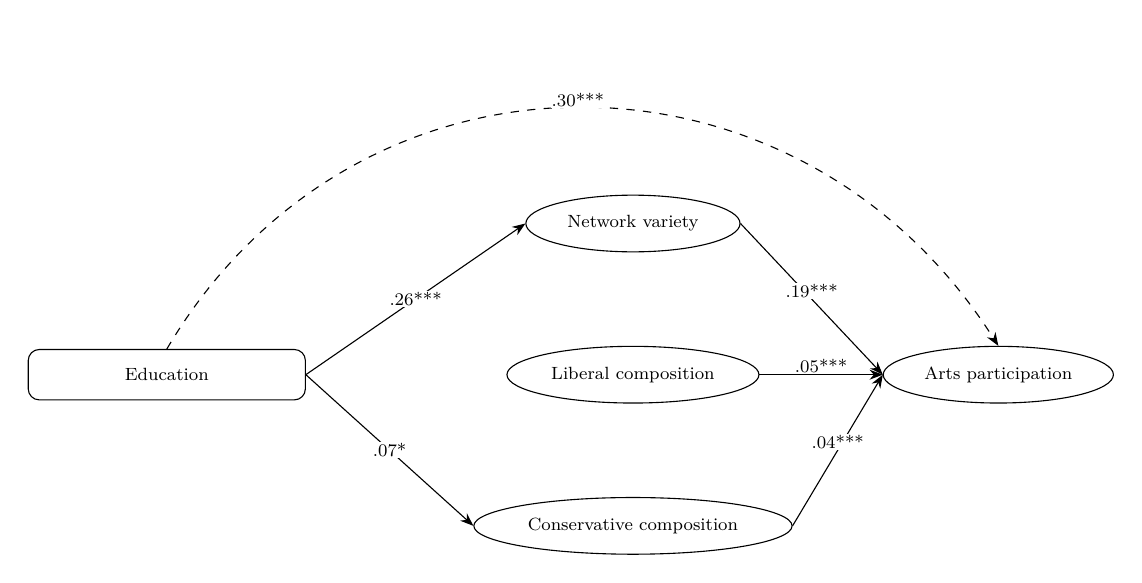
\begin{tikzpicture}[>=Stealth, font=\footnotesize, scale=0.8, transform shape,
  box/.style={draw, rounded corners, align=center, minimum width=4.4cm, minimum height=0.8cm},
  lat/.style={draw, ellipse, align=center, minimum width=3.4cm, minimum height=0.9cm},
  lab/.style={fill=white, inner sep=0.5pt, font=\footnotesize}]
\node[box] (x) at (0,0) {Education};
\node[lat] (wv) at (7.4,2.4) {Network variety};
\node[lat] (wl) at (7.4,0.0) {Liberal composition};
\node[lat] (wc) at (7.4,-2.4) {Conservative composition};
\node[lat] (act) at (13.2,0) {Arts participation};
\draw[->] (x.east) -- node[lab, pos=0.5] {.26***} (wv.west);
\draw[->] (x.east) -- node[lab, pos=0.5] {.07*} (wc.west);
\draw[->] (wv.east) -- node[lab, pos=0.5, above] {.19***} (act.west);
\draw[->] (wl.east) -- node[lab, pos=0.5, above] {.05***} (act.west);
\draw[->] (wc.east) -- node[lab, pos=0.5, above] {.04***} (act.west);
\draw[->, dashed] (x.north) .. controls (3,5.5) and (10,5.5) .. node[lab, pos=0.5, above] {.30***} (act.north);
\end{tikzpicture}
\end{center}

Note. Standardized coefficients from the weak-tie structural model with loadings fixed at the target rotation (N = 1,227). Solid arrows are paths through the network factors, dashed arrows are direct paths, and only paths significant at $p < .05$ are drawn. Asterisks follow Table 5.

\Needspace{18\baselineskip}
Figure 6. Paths from Childhood Arts Exposure to Arts Participation, Weak Ties

\begin{center}
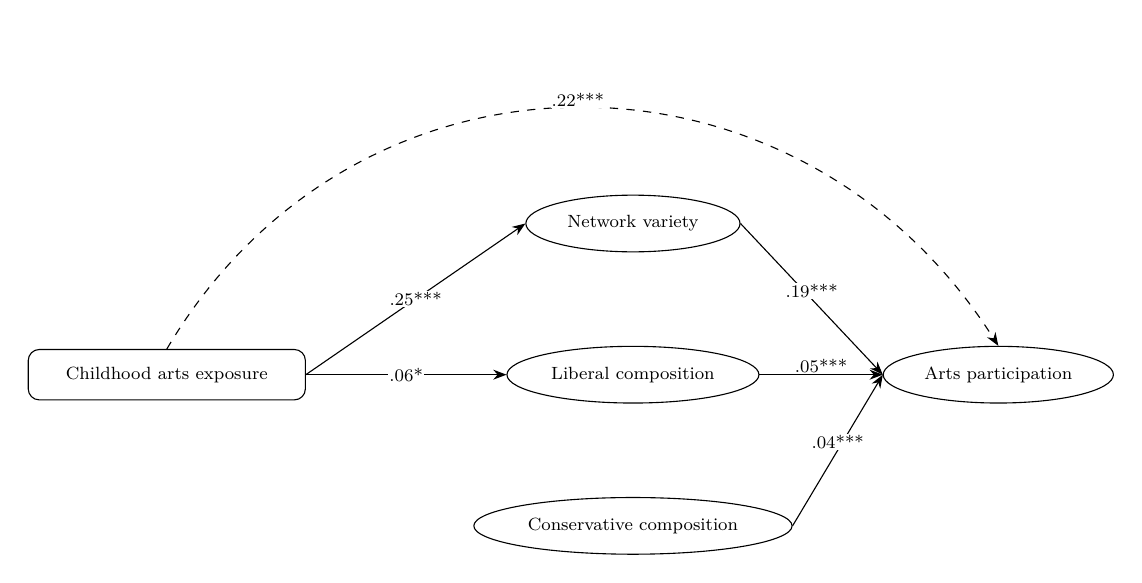
\begin{tikzpicture}[>=Stealth, font=\footnotesize, scale=0.8, transform shape,
  box/.style={draw, rounded corners, align=center, minimum width=4.4cm, minimum height=0.8cm},
  lat/.style={draw, ellipse, align=center, minimum width=3.4cm, minimum height=0.9cm},
  lab/.style={fill=white, inner sep=0.5pt, font=\footnotesize}]
\node[box] (x) at (0,0) {Childhood arts exposure};
\node[lat] (wv) at (7.4,2.4) {Network variety};
\node[lat] (wl) at (7.4,0.0) {Liberal composition};
\node[lat] (wc) at (7.4,-2.4) {Conservative composition};
\node[lat] (act) at (13.2,0) {Arts participation};
\draw[->] (x.east) -- node[lab, pos=0.5] {.25***} (wv.west);
\draw[->] (x.east) -- node[lab, pos=0.5] {.06*} (wl.west);
\draw[->] (wv.east) -- node[lab, pos=0.5, above] {.19***} (act.west);
\draw[->] (wl.east) -- node[lab, pos=0.5, above] {.05***} (act.west);
\draw[->] (wc.east) -- node[lab, pos=0.5, above] {.04***} (act.west);
\draw[->, dashed] (x.north) .. controls (3,5.5) and (10,5.5) .. node[lab, pos=0.5, above] {.22***} (act.north);
\end{tikzpicture}
\end{center}

Note. Standardized coefficients from the weak-tie structural model with loadings fixed at the target rotation (N = 1,227). Solid arrows are paths through the network factors, dashed arrows are direct paths, and only paths significant at $p < .05$ are drawn. Asterisks follow Table 5.

\Needspace{18\baselineskip}
Figure 7. Paths from Political Conservatism to Arts Participation, Weak Ties

\begin{center}
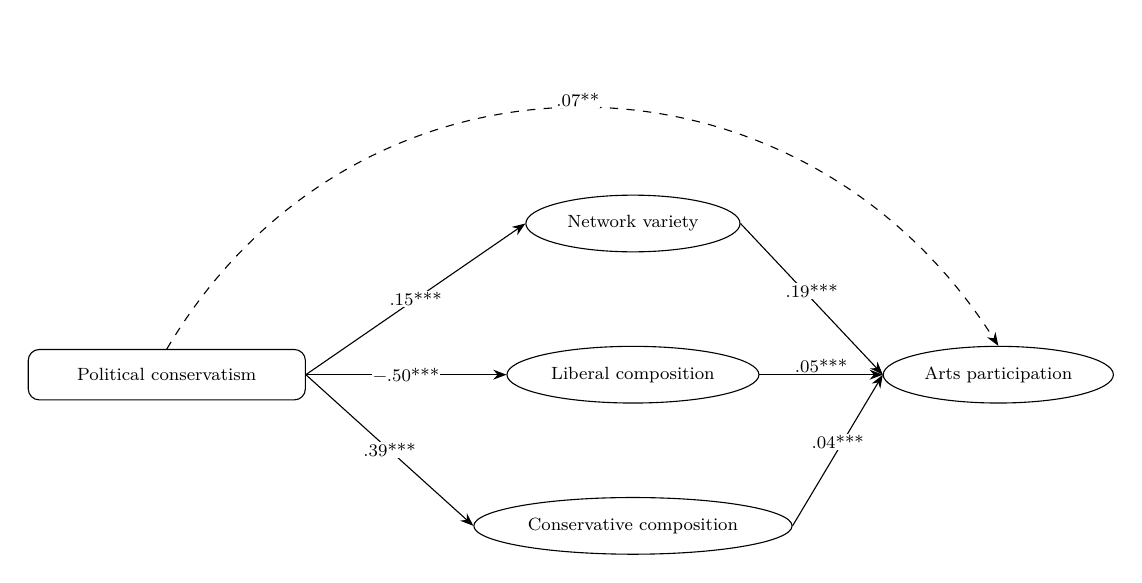
\begin{tikzpicture}[>=Stealth, font=\footnotesize, scale=0.8, transform shape,
  box/.style={draw, rounded corners, align=center, minimum width=4.4cm, minimum height=0.8cm},
  lat/.style={draw, ellipse, align=center, minimum width=3.4cm, minimum height=0.9cm},
  lab/.style={fill=white, inner sep=0.5pt, font=\footnotesize}]
\node[box] (x) at (0,0) {Political conservatism};
\node[lat] (wv) at (7.4,2.4) {Network variety};
\node[lat] (wl) at (7.4,0.0) {Liberal composition};
\node[lat] (wc) at (7.4,-2.4) {Conservative composition};
\node[lat] (act) at (13.2,0) {Arts participation};
\draw[->] (x.east) -- node[lab, pos=0.5] {.15***} (wv.west);
\draw[->] (x.east) -- node[lab, pos=0.5] {$-$.50***} (wl.west);
\draw[->] (x.east) -- node[lab, pos=0.5] {.39***} (wc.west);
\draw[->] (wv.east) -- node[lab, pos=0.5, above] {.19***} (act.west);
\draw[->] (wl.east) -- node[lab, pos=0.5, above] {.05***} (act.west);
\draw[->] (wc.east) -- node[lab, pos=0.5, above] {.04***} (act.west);
\draw[->, dashed] (x.north) .. controls (3,5.5) and (10,5.5) .. node[lab, pos=0.5, above] {.07**} (act.north);
\end{tikzpicture}
\end{center}

Note. Standardized coefficients from the weak-tie structural model with loadings fixed at the target rotation (N = 1,227). Solid arrows are paths through the network factors, dashed arrows are direct paths, and only paths significant at $p < .05$ are drawn. Asterisks follow Table 5.

\Needspace{18\baselineskip}
Figure 8. Paths from Education to Arts Participation, Strong Ties

\begin{center}
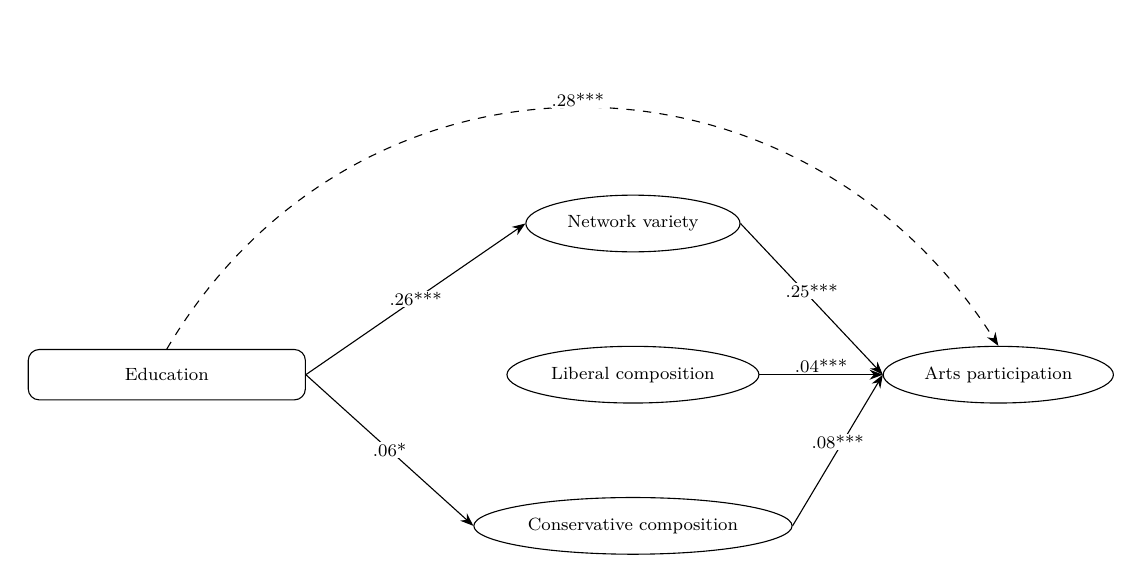
\begin{tikzpicture}[>=Stealth, font=\footnotesize, scale=0.8, transform shape,
  box/.style={draw, rounded corners, align=center, minimum width=4.4cm, minimum height=0.8cm},
  lat/.style={draw, ellipse, align=center, minimum width=3.4cm, minimum height=0.9cm},
  lab/.style={fill=white, inner sep=0.5pt, font=\footnotesize}]
\node[box] (x) at (0,0) {Education};
\node[lat] (wv) at (7.4,2.4) {Network variety};
\node[lat] (wl) at (7.4,0.0) {Liberal composition};
\node[lat] (wc) at (7.4,-2.4) {Conservative composition};
\node[lat] (act) at (13.2,0) {Arts participation};
\draw[->] (x.east) -- node[lab, pos=0.5] {.26***} (wv.west);
\draw[->] (x.east) -- node[lab, pos=0.5] {.06*} (wc.west);
\draw[->] (wv.east) -- node[lab, pos=0.5, above] {.25***} (act.west);
\draw[->] (wl.east) -- node[lab, pos=0.5, above] {.04***} (act.west);
\draw[->] (wc.east) -- node[lab, pos=0.5, above] {.08***} (act.west);
\draw[->, dashed] (x.north) .. controls (3,5.5) and (10,5.5) .. node[lab, pos=0.5, above] {.28***} (act.north);
\end{tikzpicture}
\end{center}

Note. Standardized coefficients from the strong-tie structural model with loadings fixed at the target rotation (N = 1,227). Solid arrows are paths through the network factors, dashed arrows are direct paths, and only paths significant at $p < .05$ are drawn. Asterisks follow Table 5.

\Needspace{18\baselineskip}
Figure 9. Paths from Childhood Arts Exposure to Arts Participation, Strong Ties

\begin{center}
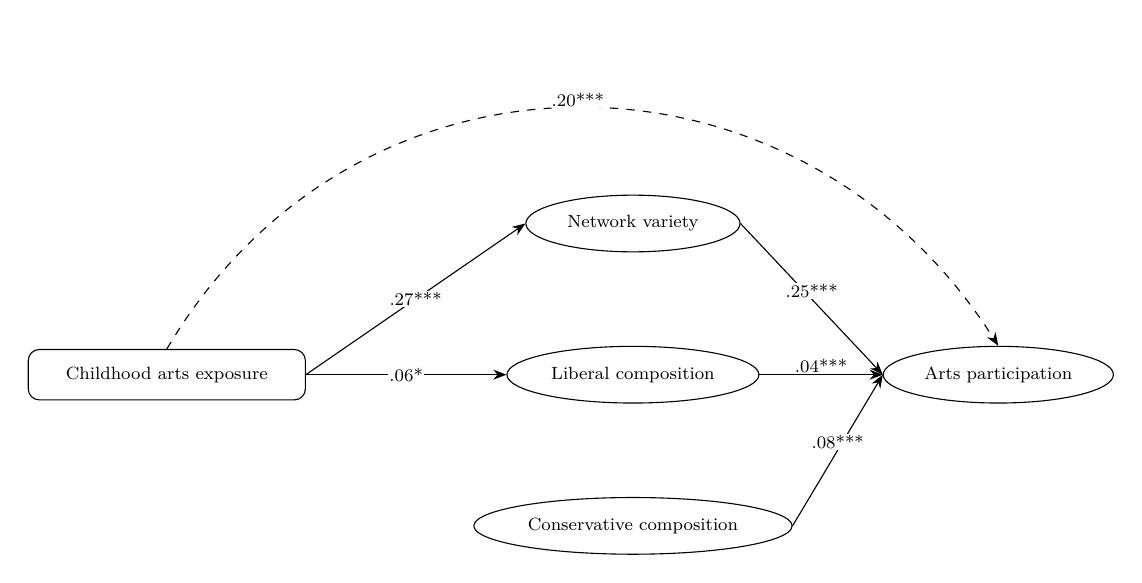
\begin{tikzpicture}[>=Stealth, font=\footnotesize, scale=0.8, transform shape,
  box/.style={draw, rounded corners, align=center, minimum width=4.4cm, minimum height=0.8cm},
  lat/.style={draw, ellipse, align=center, minimum width=3.4cm, minimum height=0.9cm},
  lab/.style={fill=white, inner sep=0.5pt, font=\footnotesize}]
\node[box] (x) at (0,0) {Childhood arts exposure};
\node[lat] (wv) at (7.4,2.4) {Network variety};
\node[lat] (wl) at (7.4,0.0) {Liberal composition};
\node[lat] (wc) at (7.4,-2.4) {Conservative composition};
\node[lat] (act) at (13.2,0) {Arts participation};
\draw[->] (x.east) -- node[lab, pos=0.5] {.27***} (wv.west);
\draw[->] (x.east) -- node[lab, pos=0.5] {.06*} (wl.west);
\draw[->] (wv.east) -- node[lab, pos=0.5, above] {.25***} (act.west);
\draw[->] (wl.east) -- node[lab, pos=0.5, above] {.04***} (act.west);
\draw[->] (wc.east) -- node[lab, pos=0.5, above] {.08***} (act.west);
\draw[->, dashed] (x.north) .. controls (3,5.5) and (10,5.5) .. node[lab, pos=0.5, above] {.20***} (act.north);
\end{tikzpicture}
\end{center}

Note. Standardized coefficients from the strong-tie structural model with loadings fixed at the target rotation (N = 1,227). Solid arrows are paths through the network factors, dashed arrows are direct paths, and only paths significant at $p < .05$ are drawn. Asterisks follow Table 5.

\Needspace{18\baselineskip}
Figure 10. Paths from Political Conservatism to Arts Participation, Strong Ties

\begin{center}
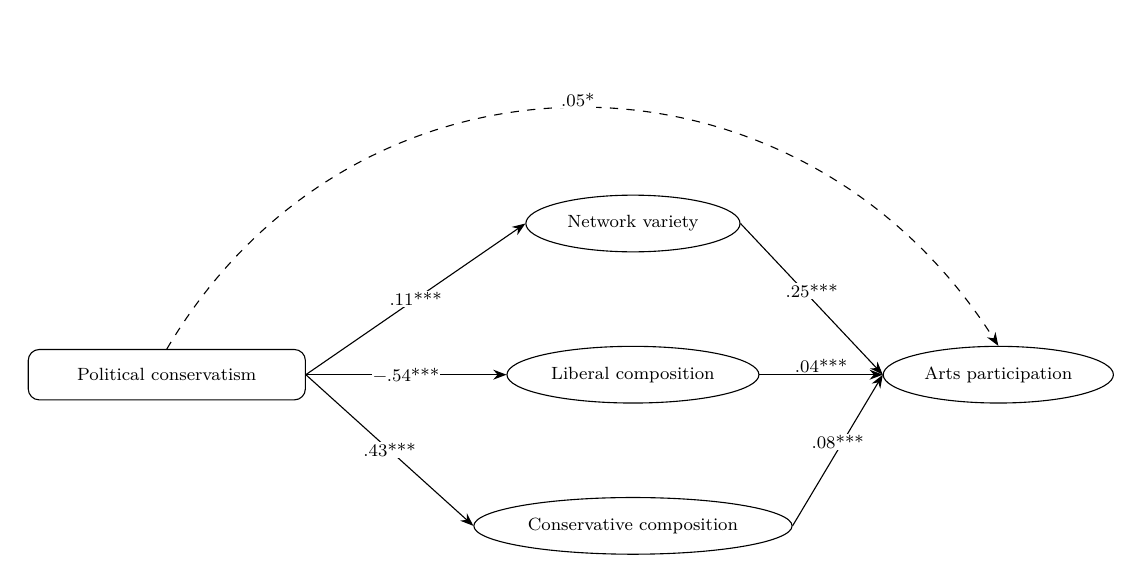
\begin{tikzpicture}[>=Stealth, font=\footnotesize, scale=0.8, transform shape,
  box/.style={draw, rounded corners, align=center, minimum width=4.4cm, minimum height=0.8cm},
  lat/.style={draw, ellipse, align=center, minimum width=3.4cm, minimum height=0.9cm},
  lab/.style={fill=white, inner sep=0.5pt, font=\footnotesize}]
\node[box] (x) at (0,0) {Political conservatism};
\node[lat] (wv) at (7.4,2.4) {Network variety};
\node[lat] (wl) at (7.4,0.0) {Liberal composition};
\node[lat] (wc) at (7.4,-2.4) {Conservative composition};
\node[lat] (act) at (13.2,0) {Arts participation};
\draw[->] (x.east) -- node[lab, pos=0.5] {.11***} (wv.west);
\draw[->] (x.east) -- node[lab, pos=0.5] {$-$.54***} (wl.west);
\draw[->] (x.east) -- node[lab, pos=0.5] {.43***} (wc.west);
\draw[->] (wv.east) -- node[lab, pos=0.5, above] {.25***} (act.west);
\draw[->] (wl.east) -- node[lab, pos=0.5, above] {.04***} (act.west);
\draw[->] (wc.east) -- node[lab, pos=0.5, above] {.08***} (act.west);
\draw[->, dashed] (x.north) .. controls (3,5.5) and (10,5.5) .. node[lab, pos=0.5, above] {.05*} (act.north);
\end{tikzpicture}
\end{center}

Note. Standardized coefficients from the strong-tie structural model with loadings fixed at the target rotation (N = 1,227). Solid arrows are paths through the network factors, dashed arrows are direct paths, and only paths significant at $p < .05$ are drawn. Asterisks follow Table 5.

Table 10. Direct, Network-Mediated, and Total Standardized Effects of Education, Childhood Arts Exposure, and Political Ideology on the Activity Factors, Weak Ties

\begin{tabular*}{\textwidth}{@{\extracolsep{\fill}}>{\raggedright\arraybackslash}p{0.36\textwidth} >{\raggedleft\arraybackslash}p{0.20\textwidth} >{\raggedleft\arraybackslash}p{0.20\textwidth} >{\raggedleft\arraybackslash}p{0.20\textwidth}@{}}
\toprule
Predictor and activity factor & Direct & Network-mediated & Total \\
\midrule
Public arts: education & \hphantom{$-$}0.30***\hphantom{***} & \hphantom{$-$}0.05***\hphantom{***} & \hphantom{$-$}0.35***\hphantom{***} \\
Public arts: childhood arts exposure & \hphantom{$-$}0.22***\hphantom{***} & \hphantom{$-$}0.05***\hphantom{***} & \hphantom{$-$}0.27***\hphantom{***} \\
Public arts: political ideology & \hphantom{$-$}0.07**\hphantom{***} & \hphantom{$-$}0.02**\hphantom{***} & \hphantom{$-$}0.09***\hphantom{***} \\
Solitary leisure: education & $-$0.01\hphantom{***} & \hphantom{$-$}0.02\hphantom{***} & \hphantom{$-$}0.01\hphantom{***} \\
Solitary leisure: childhood arts exposure & $-$0.07\hphantom{***} & \hphantom{$-$}0.03*\hphantom{***} & $-$0.04\hphantom{***} \\
Solitary leisure: political ideology & $-$0.05\hphantom{***} & $-$0.07\hphantom{***} & $-$0.12***\hphantom{***} \\
Residual: education & \hphantom{$-$}0.10*\hphantom{***} & \hphantom{$-$}0.03*\hphantom{***} & \hphantom{$-$}0.13**\hphantom{***} \\
Residual: childhood arts exposure & \hphantom{$-$}0.06\hphantom{***} & \hphantom{$-$}0.02\hphantom{***} & \hphantom{$-$}0.08*\hphantom{***} \\
Residual: political ideology & $-$0.12**\hphantom{***} & \hphantom{$-$}0.06\hphantom{***} & $-$0.07*\hphantom{***} \\
\bottomrule
\end{tabular*}

Note. Standardized effects from the labeled weak-tie model. Network-mediated effects sum the products of each predictor's path to a network factor and that factor's path to the activity factor, with standard errors from the delta method. Total effects equal direct plus network-mediated effects. * p < .05, ** p < .01, *** p < .001.

Table 11. Direct, Network-Mediated, and Total Standardized Effects of Education, Childhood Arts Exposure, and Political Ideology on the Activity Factors, Strong Ties

\begin{tabular*}{\textwidth}{@{\extracolsep{\fill}}>{\raggedright\arraybackslash}p{0.36\textwidth} >{\raggedleft\arraybackslash}p{0.20\textwidth} >{\raggedleft\arraybackslash}p{0.20\textwidth} >{\raggedleft\arraybackslash}p{0.20\textwidth}@{}}
\toprule
Predictor and activity factor & Direct & Network-mediated & Total \\
\midrule
Public arts: education & \hphantom{$-$}0.28***\hphantom{***} & \hphantom{$-$}0.07***\hphantom{***} & \hphantom{$-$}0.35***\hphantom{***} \\
Public arts: childhood arts exposure & \hphantom{$-$}0.20***\hphantom{***} & \hphantom{$-$}0.07***\hphantom{***} & \hphantom{$-$}0.27***\hphantom{***} \\
Public arts: political ideology & \hphantom{$-$}0.05*\hphantom{***} & \hphantom{$-$}0.04***\hphantom{***} & \hphantom{$-$}0.09***\hphantom{***} \\
Solitary leisure: education & \hphantom{$-$}0.02\hphantom{***} & $-$0.01\hphantom{***} & \hphantom{$-$}0.01\hphantom{***} \\
Solitary leisure: childhood arts exposure & $-$0.04\hphantom{***} & $-$0.00\hphantom{***} & $-$0.04\hphantom{***} \\
Solitary leisure: political ideology & $-$0.01\hphantom{***} & $-$0.11*\hphantom{***} & $-$0.12***\hphantom{***} \\
Residual: education & \hphantom{$-$}0.10*\hphantom{***} & \hphantom{$-$}0.03**\hphantom{***} & \hphantom{$-$}0.13**\hphantom{***} \\
Residual: childhood arts exposure & \hphantom{$-$}0.05\hphantom{***} & \hphantom{$-$}0.03*\hphantom{***} & \hphantom{$-$}0.08*\hphantom{***} \\
Residual: political ideology & $-$0.11*\hphantom{***} & \hphantom{$-$}0.04\hphantom{***} & $-$0.07*\hphantom{***} \\
\bottomrule
\end{tabular*}

Note. Standardized effects from the labeled strong-tie model, with the same definitions as Table 10. * p < .05, ** p < .01, *** p < .001.

\subsection*{Appendix: Supplementary Measurement and Robustness Models}

\Needspace{38\baselineskip}
Table A1. Oblimin-Rotated Exploratory Factor Loadings for the Activity Battery

\begin{longtable}[]{@{}
  >{\raggedright\arraybackslash}p{(\columnwidth - 8\tabcolsep) * \real{0.4200}}
  >{\raggedright\arraybackslash}p{(\columnwidth - 8\tabcolsep) * \real{0.1600}}
  >{\raggedright\arraybackslash}p{(\columnwidth - 8\tabcolsep) * \real{0.1400}}
  >{\raggedright\arraybackslash}p{(\columnwidth - 8\tabcolsep) * \real{0.1400}}
  >{\raggedright\arraybackslash}p{(\columnwidth - 8\tabcolsep) * \real{0.1400}}@{}}
\toprule
Item & Assigned target & Arts & Leisure & Residual \\
Museum & Arts & \textbf{0.84} & 0.08 & −0.10 \\
Art gallery & Arts & \textbf{0.88} & 0.03 & −0.09 \\
Symphony, orchestra, or opera & Arts & \textbf{0.95} & −0.14 & −0.11 \\
Carnival, fair, or amusement park & Arts & \textbf{0.78} & −0.02 & 0.16 \\
Music concert or festival & Arts & \textbf{0.81} & 0.01 & 0.15 \\
Play or musical & Arts & \textbf{0.86} & −0.08 & 0.00 \\
Library & Arts & \textbf{0.53} & 0.19 & −0.07 \\
Fancy restaurant & Arts & \textbf{0.64} & 0.11 & 0.29 \\
Dance performance & Arts & \textbf{0.93} & −0.20 & −0.02 \\
Movie theater & Arts & \textbf{0.64} & 0.05 & 0.37 \\
Attend sports & Arts & \textbf{0.73} & 0.05 & 0.26 \\
Hiking, camping, or boating & Arts & \textbf{0.58} & 0.26 & −0.14 \\
Historic site & Arts & \textbf{0.74} & 0.12 & −0.12 \\
Go to festival & Arts & \textbf{0.80} & 0.12 & 0.01 \\
Go for a walk & Leisure & −0.08 & \textbf{0.79} & 0.00 \\
Exercise or yoga & Leisure & 0.31 & \textbf{0.37} & 0.25 \\
Read a novel, poem, or play & Leisure & 0.35 & \textbf{0.21} & −0.11 \\
Gardening & Residual & 0.42 & 0.22 & \textbf{−0.34} \\
Fast food & Residual & 0.06 & 0.06 & \textbf{0.43} \\
Home auto repair & Residual & 0.48 & 0.16 & \textbf{−0.23} \\
\midrule
\endhead
\bottomrule
\end{longtable}

Note. Oblimin-rotated pattern loadings from an exploratory factor analysis (WLS estimation, N = 1,243). Bold entries mark each item's assigned factor. The EFA fits the 20 items adequately ($\chi^2(133) = 290.8$, $p < .001$, $\text{TLI} = .911$, $\text{RMSEA} = .080$ $[.076, .084]$). The assigned target column reports the varimax assignment used as the ESEM targets. Factor correlations from the oblique solution are .19 (arts and leisure), .15 (arts and residual), and .01 (leisure and residual).


\Needspace{26\baselineskip}
Table A2. Standardized Loadings and Antonym Residual Covariances from the Separate Weak-Tie and Strong-Tie Confirmatory Models

\begin{tabular*}{\textwidth}{@{\extracolsep{\fill}}>{\raggedright\arraybackslash}p{0.36\textwidth} l >{\raggedleft\arraybackslash}p{0.12\textwidth} l >{\raggedleft\arraybackslash}p{0.12\textwidth}@{}}
\toprule
Item & Weak factor & Loading & Strong factor & Loading \\
\midrule
Asian people & Variety & 0.83 & Variety & 0.77 \\
Second home & Variety & 0.68 & Variety & 0.71 \\
Born elsewhere & Variety & 0.78 & Variety & 0.78 \\
Middle Eastern or North African people & Variety & 0.84 & Variety & 0.86 \\
Native Hawaiian or Pacific Islander people & Variety & 0.82 & Variety & 0.83 \\
American Indian people & Variety & 0.74 & Variety & 0.81 \\
LGBTQ people & Liberal & 0.69 & Liberal & 0.71 \\
Little church & Liberal & 0.67 & Liberal & 0.67 \\
Very liberal & Liberal & 0.71 & Liberal & 0.73 \\
Hispanic or Latine people & Liberal & 0.77 & Variety & 0.73 \\
Black people & Liberal & 0.76 & Variety & 0.76 \\
City people & Liberal & 0.70 & Liberal & 0.77 \\
Lots of church & Conservative & 0.83 & Conservative & 0.83 \\
Very conservative & Conservative & 0.73 & Conservative & 0.73 \\
White people & Conservative & 0.84 & Conservative & 0.78 \\
Rural people & Conservative & 0.60 & Conservative & 0.62 \\
\midrule
Very liberal with very conservative & Residual & $-0.32$ & Residual & $-0.55$ \\
Little church with lots of church & Residual & 0.10 & Residual & $-0.05$ \\
City people with rural people & Residual & $-0.40$ & Residual & $-0.44$ \\
\bottomrule
\end{tabular*}

Note. Standardized loadings from separate three-factor WLSMV confirmatory models for weak ties and strong ties (N = 1,258 each), with the baseline models for the loadings. The residual rows come from the antonym-freed models, and each has a standard error of .02. Gender items are excluded. Item labels are abbreviated from the variable names and should be checked against the question wording.

\Needspace{30\baselineskip}
Table A3. Standardized Network-to-Activity Paths in the Separate Structural Models Under Two Rotations and in Random Halves

\begin{tabular*}{\textwidth}{@{\extracolsep{\fill}}>{\raggedright\arraybackslash}p{0.27\textwidth} >{\raggedleft\arraybackslash}p{0.11\textwidth} >{\raggedleft\arraybackslash}p{0.11\textwidth} >{\raggedleft\arraybackslash}p{0.11\textwidth} >{\raggedleft\arraybackslash}p{0.11\textwidth} >{\raggedleft\arraybackslash}p{0.11\textwidth} >{\raggedleft\arraybackslash}p{0.11\textwidth}@{}}
\toprule
 & \multicolumn{3}{c}{Target rotation} & \multicolumn{3}{c}{Oblimin rotation} \\
\cmidrule(lr){2-4}\cmidrule(lr){5-7}
Path & Full & Half A & Half B & Full & Half A & Half B \\
\midrule
Weak variety $\to$ arts & 0.19 & 0.18 & 0.20 & 0.18 & 0.17 & 0.20 \\
Weak liberal $\to$ arts & 0.05 & 0.05 & 0.04 & $-$0.01 & 0.01 & $-$0.02 \\
Weak conservative $\to$ arts & 0.04 & 0.04 & 0.04 & 0.03 & 0.02 & 0.03 \\
Weak variety $\to$ leisure & 0.07 & 0.03 & 0.12 & 0.08 & 0.05 & 0.11 \\
Weak liberal $\to$ leisure & 0.20 & 0.32 & 0.10 & 0.17 & 0.29 & 0.05 \\
Weak conservative $\to$ leisure & 0.05 & $-$0.02 & 0.15 & 0.02 & $-$0.07 & 0.14 \\
Weak variety $\to$ residual & 0.10 & 0.04 & 0.12 & $-$0.08 & $-$0.04 & $-$0.15 \\
Weak liberal $\to$ residual & $-$0.08 & $-$0.14 & 0.01 & $-$0.00 & $-$0.14 & 0.16 \\
Weak conservative $\to$ residual & $-$0.02 & $-$0.03 & $-$0.02 & $-$0.03 & $-$0.00 & $-$0.07 \\
Strong variety $\to$ arts & 0.25 & 0.24 & 0.25 & 0.23 & 0.21 & 0.25 \\
Strong liberal $\to$ arts & 0.04 & 0.05 & 0.04 & 0.01 & 0.02 & 0.00 \\
Strong conservative $\to$ arts & 0.08 & 0.08 & 0.08 & 0.05 & 0.05 & 0.04 \\
Strong variety $\to$ leisure & $-$0.05 & $-$0.10 & 0.02 & $-$0.05 & $-$0.07 & $-$0.01 \\
Strong liberal $\to$ leisure & 0.21 & 0.33 & 0.13 & 0.21 & 0.31 & 0.12 \\
Strong conservative $\to$ leisure & 0.03 & $-$0.07 & 0.17 & 0.05 & $-$0.03 & 0.16 \\
Strong variety $\to$ residual & 0.10 & 0.06 & 0.14 & $-$0.10 & $-$0.02 & $-$0.15 \\
Strong liberal $\to$ residual & $-$0.04 & $-$0.05 & 0.00 & 0.04 & $-$0.04 & 0.12 \\
Strong conservative $\to$ residual & 0.01 & $-$0.03 & $-$0.01 & $-$0.00 & $-$0.01 & $-$0.05 \\
\bottomrule
\end{tabular*}

Note. Standardized paths from separate fixed-loading WLSMV structural models (weak ties and strong ties, each with gender, education, childhood arts exposure, income, age, race and ethnicity, and political ideology as predictors). The full sample has N = 1,227; the random halves (seed 4217) have N = 600 (half A) and N = 627 (half B). The target-rotation columns match the main results in Table 5, and the oblimin columns re-estimate the loadings under an unconstrained oblimin rotation. No significance stars are shown because the halves are not designed for inference, and standard errors are in the replication output. Paths that are null in the full sample are not interpreted.


Table A4

Ordinary Least Squares Estimates of Public Arts Participation

\begin{tabular*}{\textwidth}{@{\extracolsep{\fill}}>{\raggedright\arraybackslash}p{0.40\textwidth} >{\raggedleft\arraybackslash}p{0.13\textwidth} >{\raggedleft\arraybackslash}p{0.13\textwidth} >{\raggedleft\arraybackslash}p{0.13\textwidth} >{\raggedleft\arraybackslash}p{0.13\textwidth}@{}}
\toprule
 & Model 1 & Model 2 & Model 3 & Model 4 \\
\midrule
Weak-tie variety & 0.18***\\ (0.04) & 0.10**\\ (0.04) & 0.15***\\ (0.04) & 0.09*\\ (0.04) \\
Strong-tie variety & 0.43***\\ (0.04) & 0.39***\\ (0.04) & 0.46***\\ (0.04) & 0.40***\\ (0.04) \\
Weak-tie liberal composition &  &  & $-$0.12***\\ (0.03) & $-$0.12***\\ (0.03) \\
Weak-tie conservative composition &  &  & 0.03\\ (0.04) & $-$0.01\\ (0.03) \\
Strong-tie liberal composition &  &  & 0.09**\\ (0.03) & 0.03\\ (0.03) \\
Strong-tie conservative composition &  &  & 0.13***\\ (0.04) & 0.11**\\ (0.03) \\
Man (ref. woman) &  & $-$0.00\\ (0.04) &  & $-$0.01\\ (0.04) \\
Non-binary/trans (ref. woman) &  & 0.10\\ (0.15) &  & 0.14\\ (0.14) \\
Some college (ref. high school or less) &  & 0.09\\ (0.05) &  & 0.09\\ (0.05) \\
College degree (ref. high school or less) &  & 0.37***\\ (0.06) &  & 0.37***\\ (0.06) \\
Graduate degree (ref. high school or less) &  & 0.51***\\ (0.08) &  & 0.48***\\ (0.08) \\
Childhood arts exposure &  & 0.08***\\ (0.01) &  & 0.08***\\ (0.01) \\
Household income &  & 0.01\\ (0.01) &  & 0.01\\ (0.01) \\
Age (years) &  & $-$0.01***\\ (0.00) &  & $-$0.01***\\ (0.00) \\
Black (ref. White) &  & $-$0.02\\ (0.07) &  & 0.01\\ (0.07) \\
Hispanic or Latine (ref. White) &  & $-$0.17*\\ (0.08) &  & $-$0.08\\ (0.09) \\
AAPI (ref. White) &  & $-$0.48***\\ (0.09) &  & $-$0.37***\\ (0.09) \\
Mixed/other (ref. White) &  & $-$0.27***\\ (0.06) &  & $-$0.20***\\ (0.06) \\
Political ideology (1 to 7) &  & 0.03**\\ (0.01) &  & $-$0.01\\ (0.02) \\
Intercept & $-$0.01\\ (0.02) & $-$0.45***\\ (0.11) & $-$0.01\\ (0.02) & $-$0.30*\\ (0.12) \\
\midrule
Observations & 1,227 & 1,227 & 1,227 & 1,227 \\
$R^2$ & 0.356 & 0.451 & 0.388 & 0.467 \\
\bottomrule
\end{tabular*}

Note. OLS coefficients with HC1 robust standard errors in parentheses (N = 1,227 complete cases). Outcomes are regression-method factor scores from the polychoric varimax solutions. Model 1 includes the two variety terms, Model 2 adds covariates, Model 3 adds the four composition terms, and Model 4 includes both blocks and covariates. Education enters as three dummy categories relative to high school or less. * p < .05, ** p < .01, *** p < .001.

Table A5

Ordinary Least Squares Estimates of Solitary Leisure

\begin{tabular*}{\textwidth}{@{\extracolsep{\fill}}>{\raggedright\arraybackslash}p{0.40\textwidth} >{\raggedleft\arraybackslash}p{0.13\textwidth} >{\raggedleft\arraybackslash}p{0.13\textwidth} >{\raggedleft\arraybackslash}p{0.13\textwidth} >{\raggedleft\arraybackslash}p{0.13\textwidth}@{}}
\toprule
 & Model 1 & Model 2 & Model 3 & Model 4 \\
\midrule
Weak-tie variety & 0.23***\\ (0.05) & 0.16**\\ (0.05) & 0.20***\\ (0.05) & 0.14**\\ (0.05) \\
Strong-tie variety & $-$0.19***\\ (0.05) & $-$0.19***\\ (0.05) & $-$0.13**\\ (0.05) & $-$0.16**\\ (0.05) \\
Weak-tie liberal composition &  &  & 0.14***\\ (0.04) & 0.13**\\ (0.04) \\
Weak-tie conservative composition &  &  & 0.09*\\ (0.04) & 0.06\\ (0.04) \\
Strong-tie liberal composition &  &  & 0.13**\\ (0.04) & 0.09*\\ (0.04) \\
Strong-tie conservative composition &  &  & 0.02\\ (0.04) & 0.03\\ (0.05) \\
Man (ref. woman) &  & $-$0.09\\ (0.05) &  & $-$0.05\\ (0.05) \\
Non-binary/trans (ref. woman) &  & $-$0.27\\ (0.27) &  & $-$0.22\\ (0.26) \\
Some college (ref. high school or less) &  & 0.34***\\ (0.10) &  & 0.30**\\ (0.10) \\
College degree (ref. high school or less) &  & 0.62***\\ (0.10) &  & 0.55***\\ (0.10) \\
Graduate degree (ref. high school or less) &  & 0.53***\\ (0.11) &  & 0.47***\\ (0.11) \\
Childhood arts exposure &  & 0.05*\\ (0.02) &  & 0.03\\ (0.02) \\
Household income &  & 0.02**\\ (0.01) &  & 0.02*\\ (0.01) \\
Age (years) &  & $-$0.00\\ (0.00) &  & $-$0.00\\ (0.00) \\
Black (ref. White) &  & $-$0.09\\ (0.08) &  & $-$0.03\\ (0.08) \\
Hispanic or Latine (ref. White) &  & 0.06\\ (0.11) &  & 0.06\\ (0.11) \\
AAPI (ref. White) &  & $-$0.02\\ (0.13) &  & 0.02\\ (0.13) \\
Mixed/other (ref. White) &  & 0.07\\ (0.09) &  & 0.10\\ (0.09) \\
Political ideology (1 to 7) &  & $-$0.04*\\ (0.02) &  & $-$0.01\\ (0.02) \\
Intercept & $-$0.00\\ (0.03) & $-$0.47**\\ (0.16) & $-$0.02\\ (0.03) & $-$0.50**\\ (0.16) \\
\midrule
Observations & 1,227 & 1,227 & 1,227 & 1,227 \\
$R^2$ & 0.017 & 0.089 & 0.075 & 0.121 \\
\bottomrule
\end{tabular*}

Note. OLS coefficients with HC1 robust standard errors in parentheses (N = 1,227 complete cases). Outcomes are regression-method factor scores from the polychoric varimax solutions. Model 1 includes the two variety terms, Model 2 adds covariates, Model 3 adds the four composition terms, and Model 4 includes both blocks and covariates. Education enters as three dummy categories relative to high school or less. * p < .05, ** p < .01, *** p < .001.


\end{document}
